\subsection{System/Akzeptanztests}
\label{sec:system}

Nun wollen wir am Beispiel einer Suche nach Stellenanzeigen die Entwicklung von Akzeptanztests und damit die Akzeptanztestgetriebene Softwareentwicklung (vgl. Abschnitt \ref{sec:attd} betrachten.

Zum Einsatz kommt dabei die für Systemtests entwickelte domainspezifische Sprache Cucumber, die Bereits in Abschnitt \ref{sec:cucumber} vorgestellt wurde.


\paragraph{1. Definition des gesamten Akzeptanztest}

Zusammen mit dem Kunden, oder basierend auf den Anforderungen entwickeln wir zuerst eine Spezifikation für ein Feature, und darauf aufbauend, Da die Akzeptanztests in erster Linie dazu dienen, die Software gegenüber den Anfordungen des Kunden zu validieren, und auch als Kommunikationsmittel genutzt wird, orientert sich das Vokabular an gebräuchlichen Begriffen. So ist ein einzelner Testfall ein "`Szenario"' und eine Test-Suite ein "`Feature"'. Statt "`Assertions"' (Zusicherungen) gibt es Vor- und Nachbedingungen.

Nachfolgend sei ein erstes Szenario für eine Suche nach Stellenanzeigen gezeigt.

\begin{lstlisting}
# language: de
Funktionalität: Job-Suche
  Um Jobs zu finden
  Als ein Gast
  Soll es möglich sein mittels einer Suche Jobs zu finden    
  Szenario: Auffinden durch Titel
    Angenommen wir befinden uns auf der Startseite
    Und die folgenden Jobs sind vorhanden:
       | title                    |  visible  |
       | Ruby on Rails Entwickler |   true    |
       | Java Programmierer       |   true    |
    Wenn wir "Rails" für "search" eintippen
    Und wir auf den Button "Suchen" klicken
    Dann sehen wir "Ruby on Rails Entwickler"
\end{lstlisting}

Die ersten drei Zeilen des Features ("`Funktionaliät"') beinhalten hier einen Kommentar, der lediglich die Testziele und Rahmenbedingungen definiert. Danach folgen die Testschritte. Eine Besonderheit ist der zweite: "`Und die folgenden Jobs sind vorhanden"'. Dort ermöglicht es ein Syntaxelement von Cucumber über eine Tabelle mehrere Datensätze zu definieren. Alle anderen Elemente sollten aus dem Abschnitt \ref{sec:cucumber} bereits bekannt sein.

Wenn wir dieses Feature nun ausführen, erhalten wir folgende Ausgabe:

%TODO Ausgabe TestFail
\begin{figure}[htbp]
 \centering
 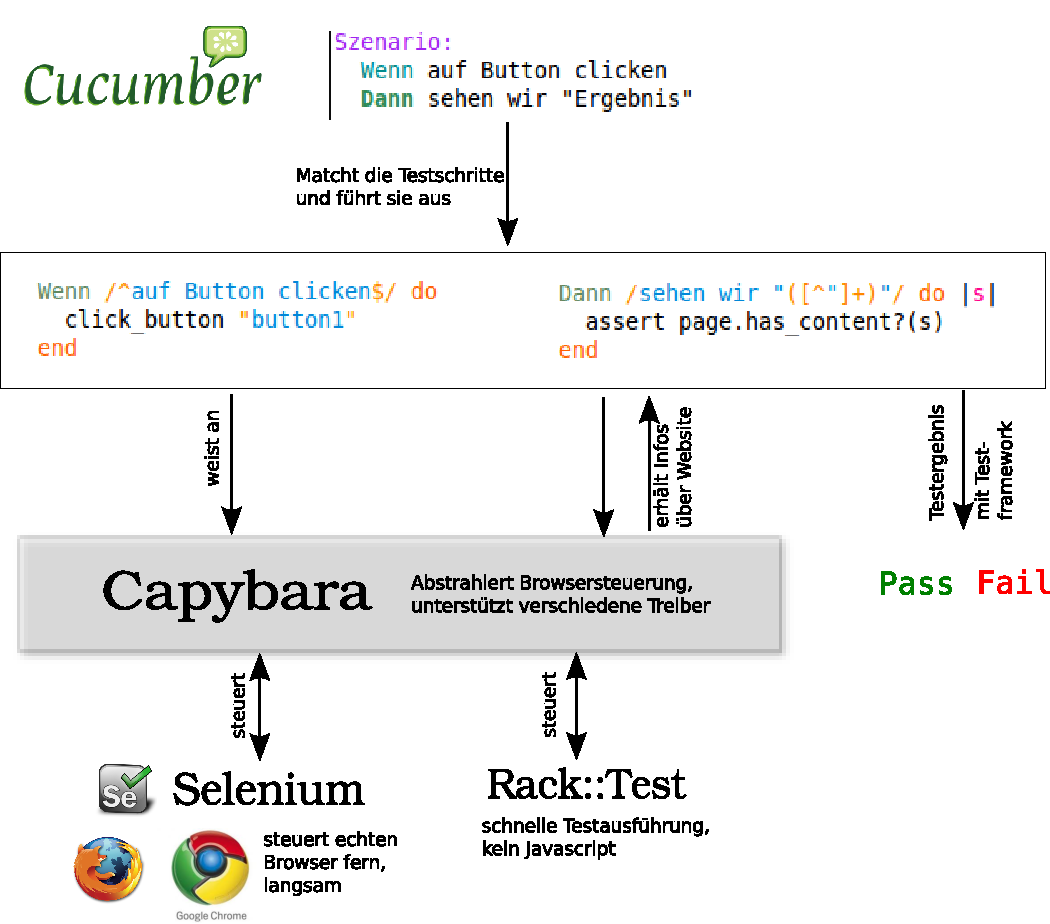
\includegraphics[width=0.9\textwidth]{./diagrams/cucumber.pdf}
 % cucumber.pdf: 595x842 pixel, 72dpi, 20.99x29.70 cm, bb=
 \caption{Ablauf beim Akzeptanztest mit Cucumber und Capybara}
 \label{fig:cucumber}
\end{figure}


Bevor wir also beginnen können das Feature zu entwickeln, müssen wir erst die Testschritte implementieren. Diese Implementierung ist i.d.R davon abhängig, welche zugrunde liegende Methode man verwendet, einen Browser zu simulieren, und welches Test-Framework für Zusicherungen benutzt wird. Wir haben uns für Capybara entschieden, welches sehr flexibel bei der Wahl der Browser-Engine ist, und für die Definition der Zusicherungen für das schon bekannte Test::Unit. Der Ablauf des Akzeptanztest ist in Abbildung \ref{fig:cucumber} abgebildet. 
Die Anweisungen des Akzeptanztests werden auf die definierten Testschritte gemappt, die Cucumber dann sequentiell ausführt. 

Hier zuerst die Basis-Testschritte, die für fast jedes Feature benötigt werden. Falls wir die englische Testschrittdefinition nutzen, entfällt dieser Schritt, da Capybara bereits häufig gebrauchte Testschritte mitliefert.

\begin{lstlisting}
Angenommen /^wir befinden uns auf der Startseite$/ do 
  visit "/"
end
Wenn /^wir "([^"]*)" für "([^"]*)" eintippen$/ do |text, input_name|
  fill_in input_name, :with => text
end
Und /^wir auf den Button "([^"]*)" klicken$/ do |text|
  click_button text
end

Dann /^sehen wir "([^"]*)"$/ do |string|
  assert page.has_content?(string)
end
\end{lstlisting}
Der erste Testschritt gibt unserem simulierten Browser die Anweisung, die Startseite zu besuchen. Der Zweite Testschritt spezifiziert  einen Testschritt mit 2 variablen Texten, die an unseren Block mit übergeben werden. Wir möchten, dass der erste Begriff in "`..."' als Text in ein Formularelement mit dem Bezeichner des zweiten Begriffes eingetragen wird.
Der Dritte implementiert den Klick auf einen HTML-Button mit dem angegebenen Inhalt. 
Während die ersten 3 Schritte Aktionen ausführen, hat der 4. eine andere Funktion: Er spezifiert eine Zusicherung, dass auch unserer aktuellen Webseite irgendwo ein gewisser Inhalt steht.


\begin{lstlisting}
# table.hashes ->
#  [ {:title => "Ruby on Rails Entwickler",  :visible => true},
#    {:title => "Java Programmierer",        :visible => true}]
Angenommen /^die folgenden Jobs sind vorhanden:$/ do |table|
  valid_job = jobs(:visible_job).attributes
  table.hashes.each do |hash|
    attributes = valid_job.merge(hash)
    Job.create(attributes)
  end
end
\end{lstlisting}
Der Testschritt für die Implementation des Testschrittes mit der Tabelle, ist etwas umfangreicher. Wir bekommen von Cucumber ein Array von Hashes übergeben, die die geparste Tabelle beinhaltet. Über diese können wir nun mit dem Iterator "`each"' iterieren, und die definierten Attribute mit denen unserer Job-Fixture\footnote{Anmerkung: Für diese Aufgabe eignen sich Factories deutlich besser. Da mit Fixtures schon eine Testdatengenerierung eingeführt wurde, bleiben wir aber aus Konsistenzgründen dabei.} vereinigt wird, um somit einen neuen Job in der Testdatenbank anzulegen. Wir haben den Testschritt so allgemein gehaltet, dass wir ihn in späteren Szenarien gut verwenden können, um weitere Jobs mit speziellen Attributen zu generieren.

Nun können wir Cucumber erneut ausführen, und das Ergebnis ist ein anderes:

% TODO Ausgabe TestFail

\tddred
Der Test schlug also fehl, da noch kein Suchfeld eingebaut wurde. Dies erreichen wir, indem wir auf der View der Startseite eines einbauen:

\begin{lstlisting}
<%= form_tag "/jobs" do %>
  <%= text_field_tag(:search) %>
  <%= submit_tag("Suchen") %>
<% end %> 
\end{lstlisting}
Wir implementieren in der View der Startseite ein Suchfeld mit den Form-Hilfsfunktionen, die Rails anbietet. Dabei verwenden wir hier ERB, eine Template-Sprache, die normalerweise HTML-Code generiert, und es ermöglicht innerhalb der "`\verb|<%= ... \%>|"' Ruby Code auszuführen.

Jetzt folgt die Implementierung der Suche im Jobs-Controller:

\begin{lstlisting}
class JobsController
  def index
    @jobs = Job.where("title like ?", "%#{params[:search]}%")
  end
end
\end{lstlisting}
Im Jobs-Controller implementieren wir die Bereitstellung der Jobs mittels einer Datenbankabfrage. Dabei nutzen wir die Datenbankfunktion von ActiveRecord und führen eine partielle Match-Suche der Suchparameter über die Tabellenspalte "`title"' aus. Das Ergebnis speichern wir in der Instanzvariable jobs, und stellen es so der View zur Verfügung.

\begin{lstlisting}
<% @jobs.each do |job| %>
  <div class='job'>
    <h3><%= job.title %></h3>
  </div>
<% end %>
\end{lstlisting}

Damit nun der Test besteht, muss als letztes noch eine View implementiert werden, die (zumindest) die Titel aller in der Suche gefundenen Jobs ausgibt, hier z.B. als Überschrift.
\tddgreen

% TODO test passed

Auch innerhalb der Akzeptanztestgetriebenen Entwicklung ist Refaktorisieren ein fester Bestandteil innerhalb des Entwicklungszyklus.
Ein guter Ansatz wäre z.B. die Suchlogik aus dem Controller in die Job-Modelklasse auszulagern.

\tddrefactor
\begin{lstlisting}
class Job
  ...
  def self.perform_search(params)
    where("title like ?", "#{params[:search]}") 
  end
\end{lstlisting}
Wir lagern die Suchmethode in eine neue Klassenmethode der Job-Klasse aus.

\begin{lstlisting}
class JobsController
  def index
    @jobs = Job.perform_search(params)
  end
end
\end{lstlisting}
Nun können wir die neu implementierte Funktion in unserem Controller verwenden.

\paragraph{Ausblick}
Nun haben wir ein erstes Szenario mit Cucumber implementiert. Da wir schon ein paar Testschritte implementiert haben, ist die Entwicklung von weiteren Szenarien leichter. 
Die Tests wurden bisher durch einen simulierten Browser RackTest ausgeführt. Da wir Capybara als Abstraktion des Browsers genutzt haben, wäre eine Umstellung auf eine reale Browserumgebung, z.B: Firefox oder Chrome, kein Problem. Deren Ausführung ist zwar deutlich langsamer als bei RackTest, dafür findet hier der Test unter realen Bedingungen, nämlich in einem Browser, wie ihn auch später Nutzer der Web-Anwendung besitzen.
